\documentclass{beamer}
\usepackage[utf8]{inputenc}
\usepackage[russian]{babel}
\usepackage{amsmath,mathrsfs,mathtext}
\usepackage{graphicx, epsfig}
\usepackage{placeins}
\usetheme{Warsaw}%{Singapore}%{Warsaw}%{Warsaw}%{Darmstadt}
\usecolortheme{sidebartab}
\setlength\headheight{10pt}
\definecolor{beamer@blendedblue}{RGB}{15,120,80}
%----------------------------------------------------------------------------------------------------------
\title[\hbox to 56mm{Тематический поиск схожих дел\hfill\insertframenumber\,/\,\inserttotalframenumber}]
{Тематический поиск схожих дел в коллекции актов арбитражных судов}
\author[Н.\,А. Герасименко]{\large \\Герасименко Николай Александрович}
\institute{\large
Московский авиационный институт}

\date{\footnotesize{\emph{Курс:} Численные методы обучения по прецедентам\par (практика, В.\,В. Стрижов)/Группа 8О-103М, весна 2019}}
%----------------------------------------------------------------------------------------------------------
\begin{document}
%----------------------------------------------------------------------------------------------------------
\begin{frame}
%\thispagestyle{empty}
\titlepage
\end{frame}
%-----------------------------------------------------------------------------------------------------
\begin{frame}{Цель исследования}
\begin{block}{Цель работы}
	Решение задачи информационного поиска по коллекции актов арбитражных судов.
    \end{block}
\begin{block}{Проблема}
	Специалисты в области юриспруденции вынуждены тратить большое количество времени на поиск релевантной судебной практики.
    \end{block}
\begin{block}{Метод решения}
	Построение тематической модели коллекции с помощью открытой библиотеки BigARTM, реализующей вероятностное тематическое моделирование на основе аддитивной регуляризации.
    \end{block}
\end{frame}
%----------------------------------------------------------------------------------------------------------
\begin{frame}{Литература}
Теория АРТМ:
    \begin{itemize}
        \item Konstantin Vorontsov and Anna Potapenko. Additive regularization of topic models. Machine Learning, 2015.
    \end{itemize} 
Библиотека BigARTM:
    \begin{itemize}
        \item Konstantin Vorontsov, Oleksandr Frei, Murat Apishev, Peter Romov, and Marina Dudarenko. Bigartm: open source library for regularized multimodal topic modeling of large collections.
In International Conference on Analysis of Images, Social Networks and Texts, pages 370-381. Springer, 2015.
    \end{itemize} 
Опорное исследование:
    \begin{itemize}
        \item Anastasia Ianina, Lev Golitsyn, and Konstantin Vorontsov. Multi-objective topic modeling for exploratory search in tech news. In Communications in Computer and Information Science, pages 181-193. Springer International Publishing, nov 2017.
    \end{itemize} 
\end{frame}
%----------------------------------------------------------------------------------------------------------
\begin{frame}{Постановка задачи}
\begin{block}{Дано}
%$(d_{i},w_{i},t_{i})_{i=1}^{n} \sim p(d,w,t)$, где
	Коллекция текстовых документов $D$
    \begin{itemize}
        \item $n_{dw}$ - частоты терминов $w$ в документах коллекции $d \in D$.
    \end{itemize} 
    \end{block}
\begin{block}{Найти}
	Параметры тематической модели $p(w|d)=\sum\limits_{t \in T} {\phi_{wt}\theta_{td}}$
    \begin{itemize}
        \item $\phi_{wt}$ - вероятности терминов $w$ в темах $t \in T$.
        \item $\theta_{td}$ - вероятности тем $t$ в каждом документе $d \in D$.
    \end{itemize} 
	Максимизируя логарифм правдоподобия с регуляризаторами:
\begin{align*}
	\sum\limits_{d,w} {n_{dw}ln\sum\limits_{t \in T}} {\phi_{wt}\theta_{td}}+\sum\limits_{i}\tau_{i}R_{i}(\Phi,\Theta)\to \max
\end{align*} 
    \end{block}
%\begin{block}{Внешний критерий качества}
%	Специалисты в области юриспруденции вынуждены тратить большое количество времени на поиск релевантной судебной практики.
   % \end{block}
\end{frame}
%----------------------------------------------------------------------------------------------------------
\begin{frame}{Внешний критерий качества}
\begin{block}{Используемая информация}
	Для оценки качества построения векторных представлений документов коллекции используем информацию о принадлежности каждого документа определенной категории дел таких как, например, <<Особенности банкротства отдельных категорий должников>> или <<Внешнее управление>>.
    \end{block}
\begin{block}{Идея}
	Рассчитав согласованность картины кластеризации векторных предствлений документов с картиной принадлежности документов их категориям, получаем оценку адекватности векторных предствлений. 
    \end{block}
\begin{block}{Критерии согласованности}
    \begin{itemize}
        \item Adjusted Rand Index (ARI).
        \item Adjusted Mutual Information (AMI).
    \end{itemize} 
    \end{block}
 
\end{frame}
%----------------------------------------------------------------------------------------------------------
\begin{frame}{Необходимость регуляризаторов}
\begin{block}{Оптимизационная задача в АРТМ}
	В соответствии с теорией аддитивной регуляризации тематических моделей для каждой модальности вводится критерий логарифма правдоподобия и с помощью EM-алгоритма максимизируется их взвешенная сумма.
    \end{block}
\begin{block}{Регуляризаторы $R_{i}$}
	Добавляются к сумме как дополнительные критерии c \\*весами $\tau_{i}$, необходимые поскольку в общем случае задача имеет бесконечно много решений.
\begin{align*}
	\sum\limits_{d,w} {n_{dw}ln\sum\limits_{t \in T}} {\phi_{wt}\theta_{td}}+\sum\limits_{i}\tau_{i}R_{i}(\Phi,\Theta)\to \max
\end{align*} 
    \end{block}
\end{frame}
%----------------------------------------------------------------------------------------------------------
\begin{frame}{Используемые регуляризаторы \\*Регуляризаторы сглаживания и разреживания}
\begin{block}{Общий вид}
	Данные два регуляризатора имеют одинаковый вид и отличаются только знаками коэффициентов $\alpha$ и $\beta$, для регуляризатора разреживания они отрицательны.
\begin{align*}
R(\Phi,\Theta)=\beta \sum_{m \in M}\sum_{t \in T}\sum_{w \in W^m} \beta_{w} ln \phi_{wt} + \alpha \sum_{d \in D}\sum_{t \in T}\alpha_{t} ln\theta_{td}\to \max.
\end{align*} 
    \end{block}
\begin{block}{Назначение}
Регулятор сглаживания вводит в модель требование схожести распределений $\phi_{wt}$ с распределением $\beta_{w}$ и $\theta_{td}$ с распределением $\alpha_{t}$. Регуляризатор разреживания, в свою очередь, способствует появлению нулевых элементов в распределенях $\phi_{wt}$ и $\theta_{td}$, что позволяет находить более компактные представления документов.
    \end{block}
\end{frame}
%----------------------------------------------------------------------------------------------------------
\begin{frame}{Используемые регуляризаторы \\*Регуляризатор декоррелирования}
\begin{block}{Общий вид}
\begin{align*}
R(\Phi)=-\tau \sum_{t \in T}\sum_{s \in T\backslash t}\sum_{w \in W} \phi_{wt}\phi_{ws} \to max.
\end{align*} 
    \end{block}
\begin{block}{Назначение}
Вводит в модель требование различности тем путем минимизации ковариации между столбцами матрицы $\Phi$. Также побочным эффектом работы регуляризатора декоррелирования является разреживание матрицы $\Phi$, поэтому в случае его применения, можно не применять регуляризатор разреживания для нее.
    \end{block}
\end{frame}
%----------------------------------------------------------------------------------------------------------
\begin{frame}{Стратегия регуляризации}
\end{frame}
%----------------------------------------------------------------------------------------------------------
\begin{frame}{Результаты вычислительного эксперимента \\*Внутренние критерии качества.}
\vspace{0.01em}
\begin{figure}
      \vspace{0.01em}
        Зависимости перплексии и разреженности распределений терминов в темах \begin{tabular}{cc}
        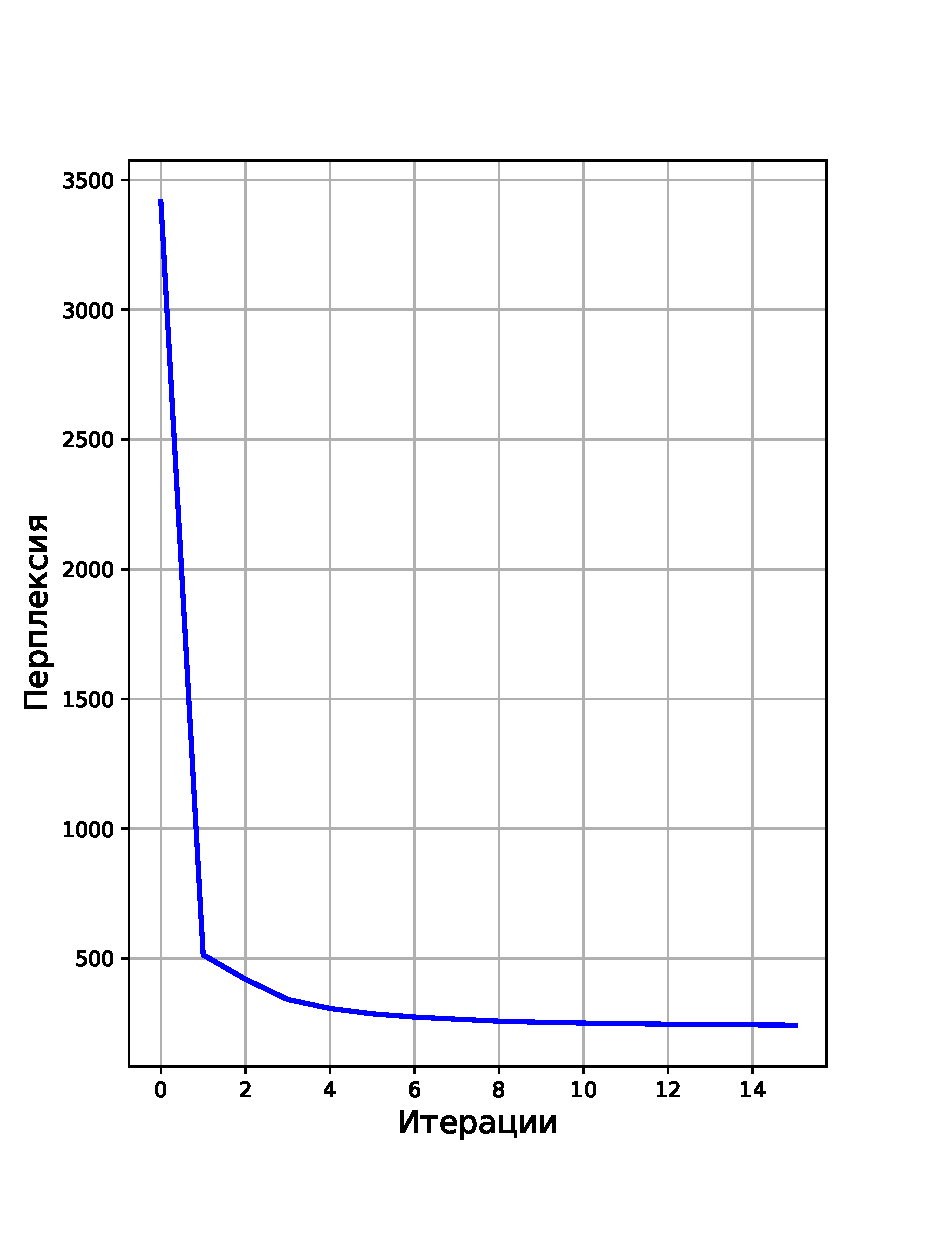
\includegraphics[width=5cm]{perplexity}
         &
         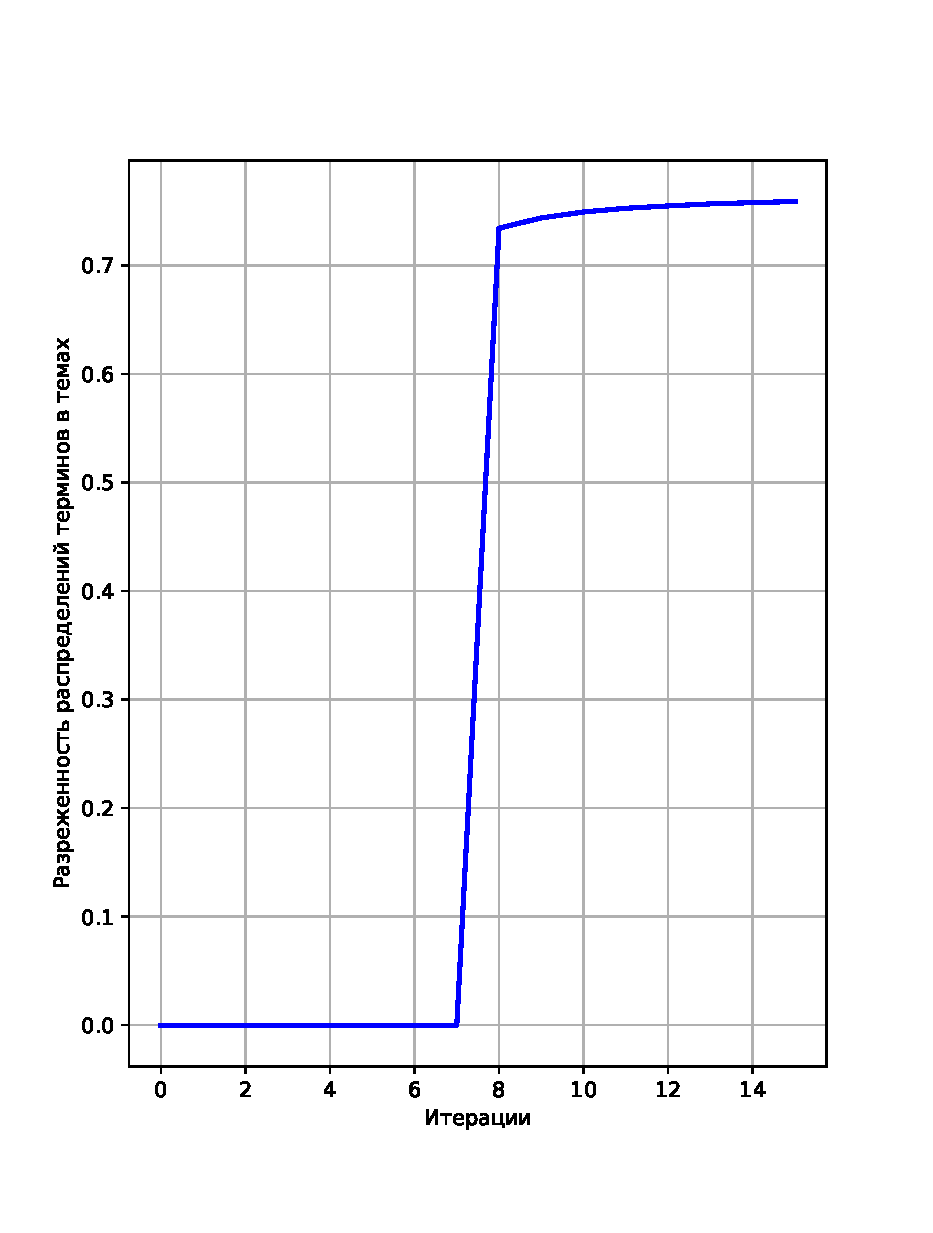
\includegraphics[width=5cm]{sparseTheta}
         \end{tabular}
\label{fg:Example}
\end{figure}
%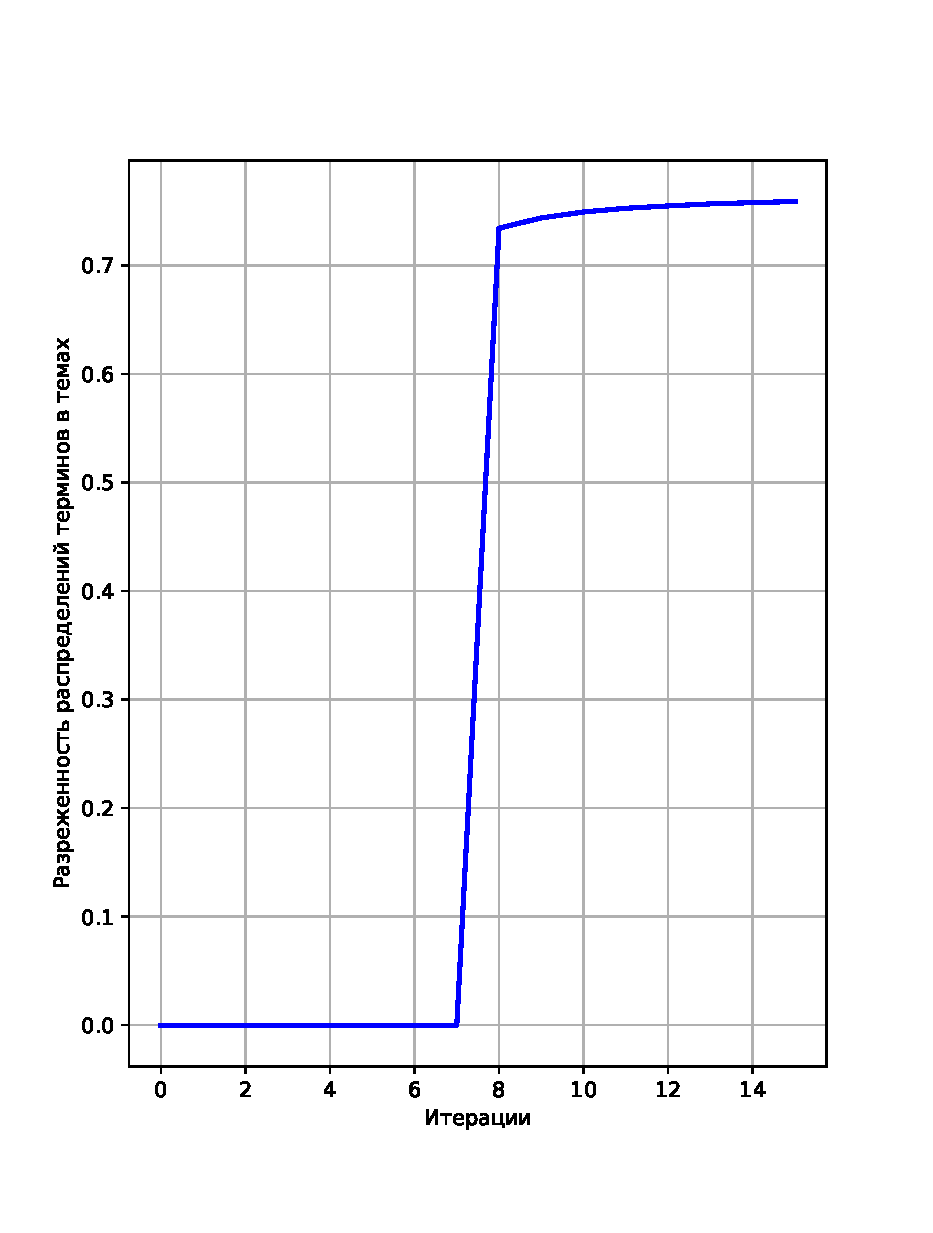
\includegraphics[width=0.5\textwidth]{sparseTheta}
%\\ Зависимости перплексии и разреженности распределений терминов в темах.
\end{frame}
%----------------------------------------------------------------------------------------------------------
\begin{frame}{Результаты вычислительного эксперимента \\*Внешние критерии качества.}
\begin{block}{Сравнение с базовыми алгоритмами}
	Для оценки качества модели были использованы в качестве базовых алгоритмов  
    \begin{itemize}
        \item TF-IDF по словам 
        \item TF-IDF по выделенным из текста ссылкам на нормативно-правовые акты (НПА), например, \\*<<пункт 3 статьи 6 УК РФ>>.
    \end{itemize} 
    \end{block}

\begin{table}[H]
% \caption{\label{tab:summary}Сравнение показателей внешнего критерия качества.}
\begin{center}
\begin{tabular}{|c|c|c|}
\hline
Модель & ARI & AMI\\
\hline
TF-IDF по словам & 10\% & 12.5\% \\
\hline
TF-IDF по ссылкам на НПА & 17\% & 22\% \\
\hline
АРТМ & 37.5\% & 42\% \\
\hline
\end{tabular}
\end{center}
\end{table}
\end{frame}
%----------------------------------------------------------------------------------------------------------
\begin{frame}{Заключение}
\end{frame}
%----------------------------------------------------------------------------------------------------------
\end{document} 